\section{Analisi delle performance}
\label{cap:performance-analysis}

\subsection{Domanda \#1}

\begin{displayquote}
Eseguite i tre algoritmi che avete implementato (Prim, Kruskal Naive e Kruskal efficiente) sui grafi del dataset. Misurate i tempi di calcolo dei tre algoritmi e create un grafico che mostri la variazione dei tempi di calcolo al variare del numero di vertici nel grafo. Per ognuna delle istanze del problema, riportate il peso del minimum spanning tree ottenuto dagli algoritmi.
\end{displayquote}

\noindent Le tabelle \ref{table:KruskalNaive-results},
 \ref{table:KruskalUnionFind-results}, \ref{table:KruskalUnionFindCompressed-results}
 e \ref{table:PrimBinaryHeap-results} in appendice \ref{cap:runtime-tables} riportano i risultati dell'MST ottenuto dagli algoritmi e il loro tempo di esecuzione per ogni file di input. \\

\noindent I seguenti grafici mostrano la variazioni delle performance temporali degli algoritmi rispetto al numero di nodi del grafico. Non abbiamo incluso il numero di edges poiché tutti i grafi in input erano sparsi, ovvero gli archi non erano mai più numerosi di un fattore 1.4 rispetto al numero di vertici, quindi tale dato non avrebbe aggiunto informazioni. Le figure \ref{fig:TheThreeComparison300}, \ref{fig:TheThreeComparison1k}
e \ref{fig:TheThreeComparison2k} mostrano una comparativa piuttosto significativa tra i tre algorimti.
\'E possibile notare infatti che anche con taglie dell'input molto piccole il comportamento degli
algorimti differisce in modo cosistente: in particolare, KruskalNaive assume sin da subito un
andamento esponenziale nel numero di nodi, e non compete per nulla con KruskalUnionFind e PrimBinaryHeap.

\begin{figure}[H]
    \centering
    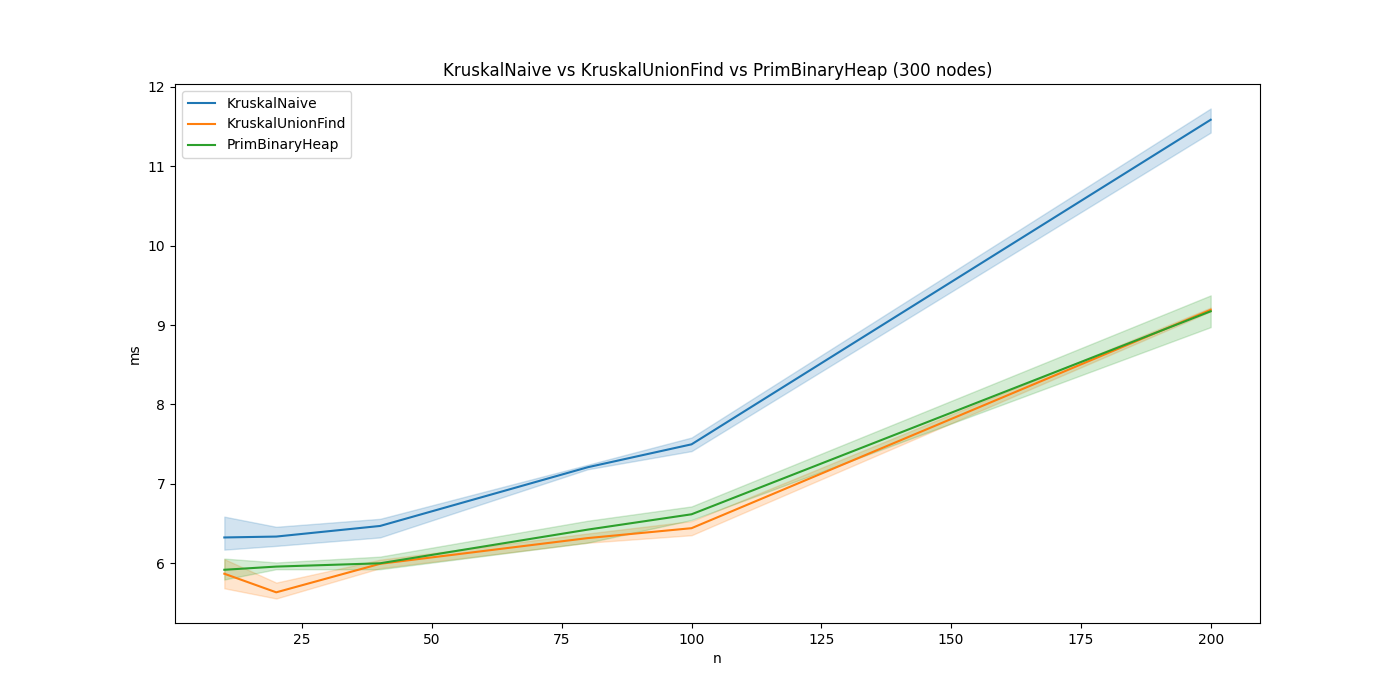
\includegraphics[width=0.9\textwidth]{./images/KruskalNaive_vs_KruskalUnionFind_vs_PrimBinaryHeap_(300_nodes).png}
	\caption{Andamento di KruskalNaive, KruskalUnionFind, PrimBinaryHeap con taglia dell'input da 0 a 300 nodi.}
    \label{fig:TheThreeComparison300}
\end{figure}

\begin{figure}[H]
    \centering
    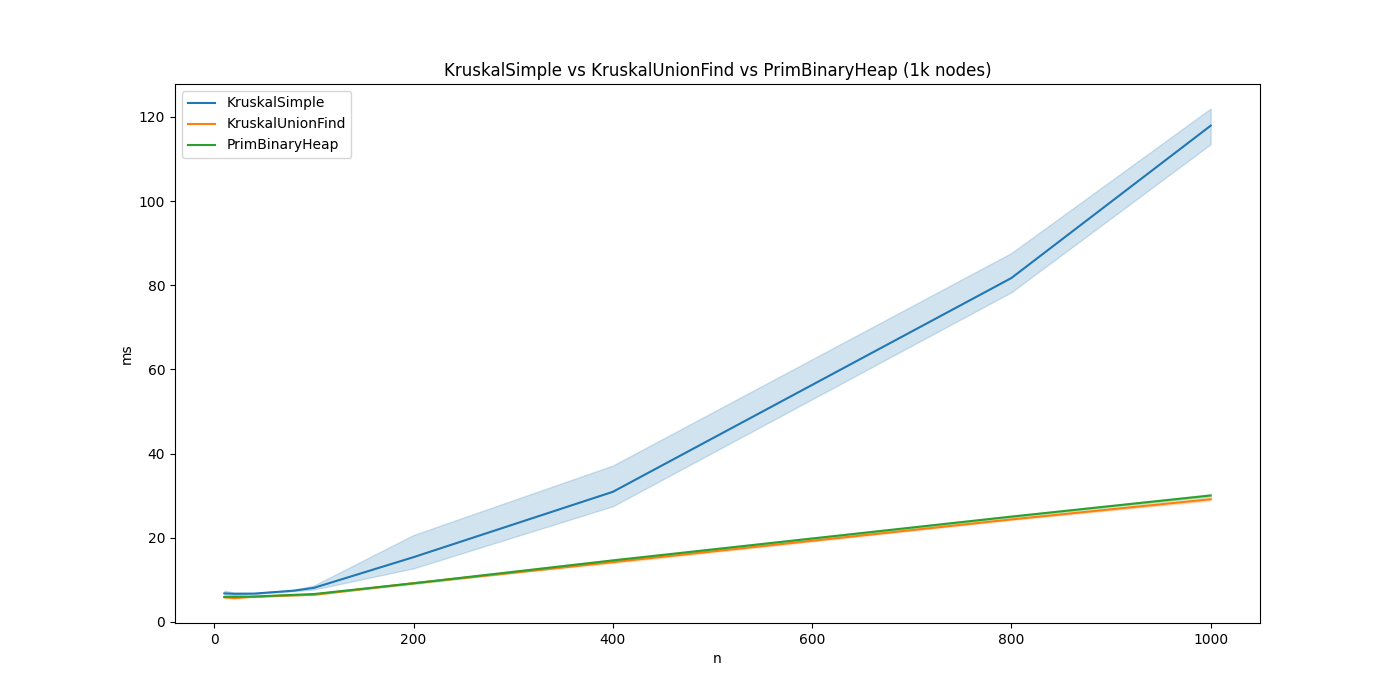
\includegraphics[width=0.9\textwidth]{./images/KruskalNaive_vs_KruskalUnionFind_vs_PrimBinaryHeap_(1k_nodes).png}
    \caption{Andamento di KruskalNaive, KruskalUnionFind, PrimBinaryHeap con taglia dell'input da 0 a 1000 nodi.}
    \label{fig:TheThreeComparison1k}
\end{figure}

\begin{figure}[H]
    \centering
    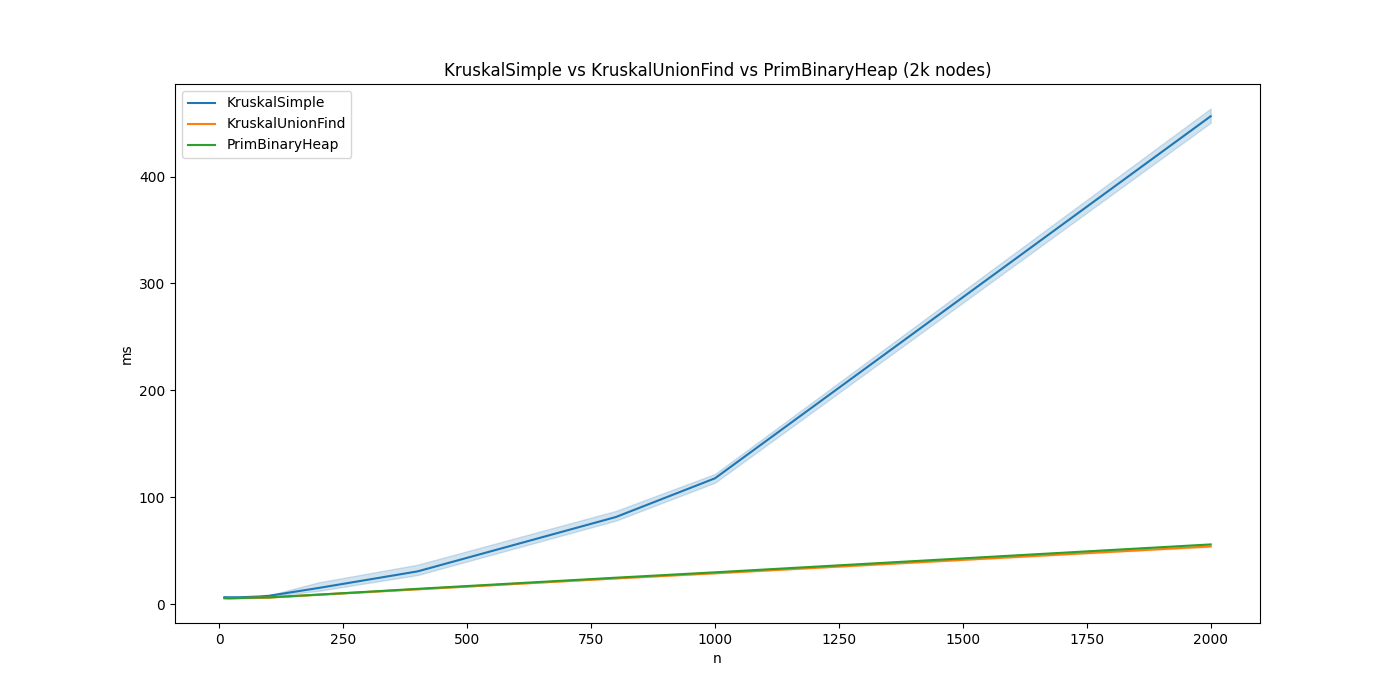
\includegraphics[width=0.9\textwidth]{./images/KruskalNaive_vs_KruskalUnionFind_vs_PrimBinaryHeap_(2k_nodes).png}
    \caption{Andamento di KruskalNaive, KruskalUnionFind, PrimBinaryHeap con taglia dell'input da 0 a 2000 nodi.}
    \label{fig:TheThreeComparison2k}
\end{figure}

\noindent Per quanto riguarda KruskalUnionFind e PrimBinaryHeap la differenza è più sottile,
e viene mostrata dalle figure \ref{fig:TheTwoComparison2k} e \ref{fig:TheTwoComparison5k}, ma è molto facile
vedere che a meno di un piccolo fattore i due hanno lo stesso trend di crescita.

\begin{figure}[H]
    \centering
    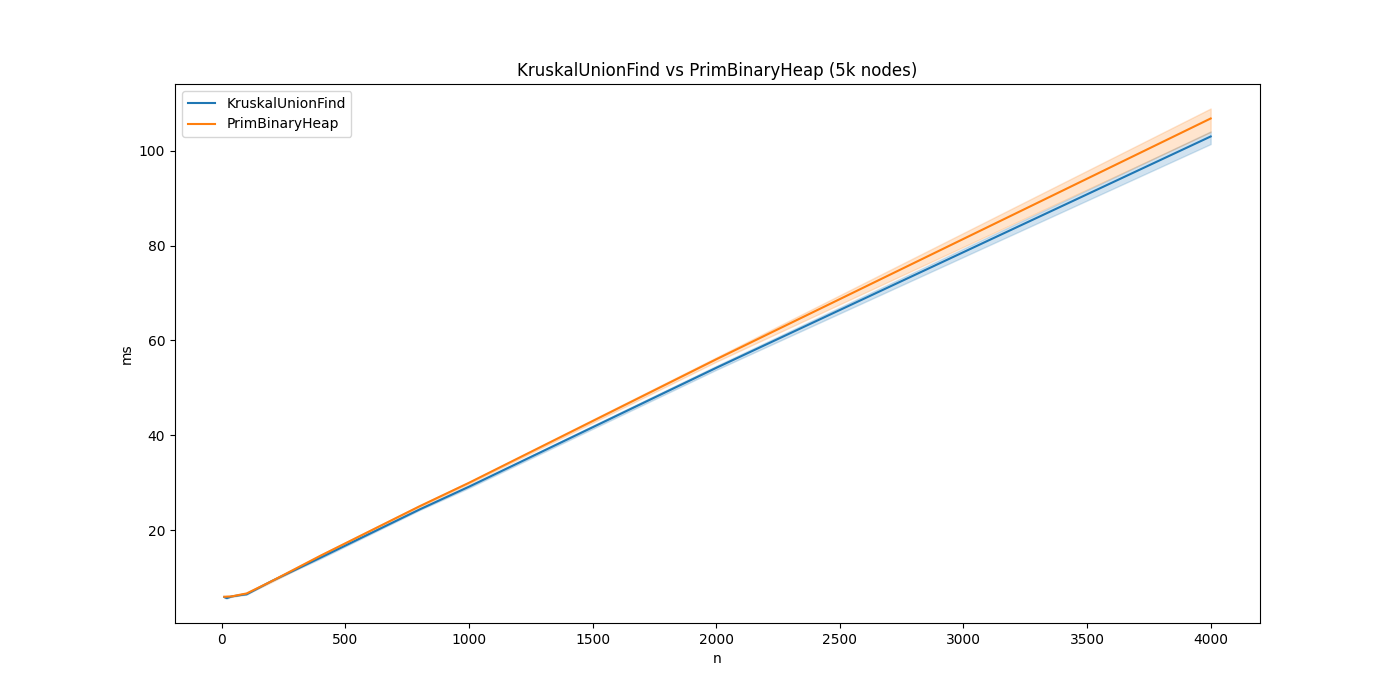
\includegraphics[width=1.0\textwidth]{./images/KruskalUnionFind_vs_PrimBinaryHeap_(5k_nodes).png}
	\caption{Andamento di KruskalUnionFind e PrimBinaryHeap con taglia dell'input da 0 a 2000 nodi.}
    \label{fig:TheTwoComparison2k}
\end{figure}

\begin{figure}[H]
    \centering
    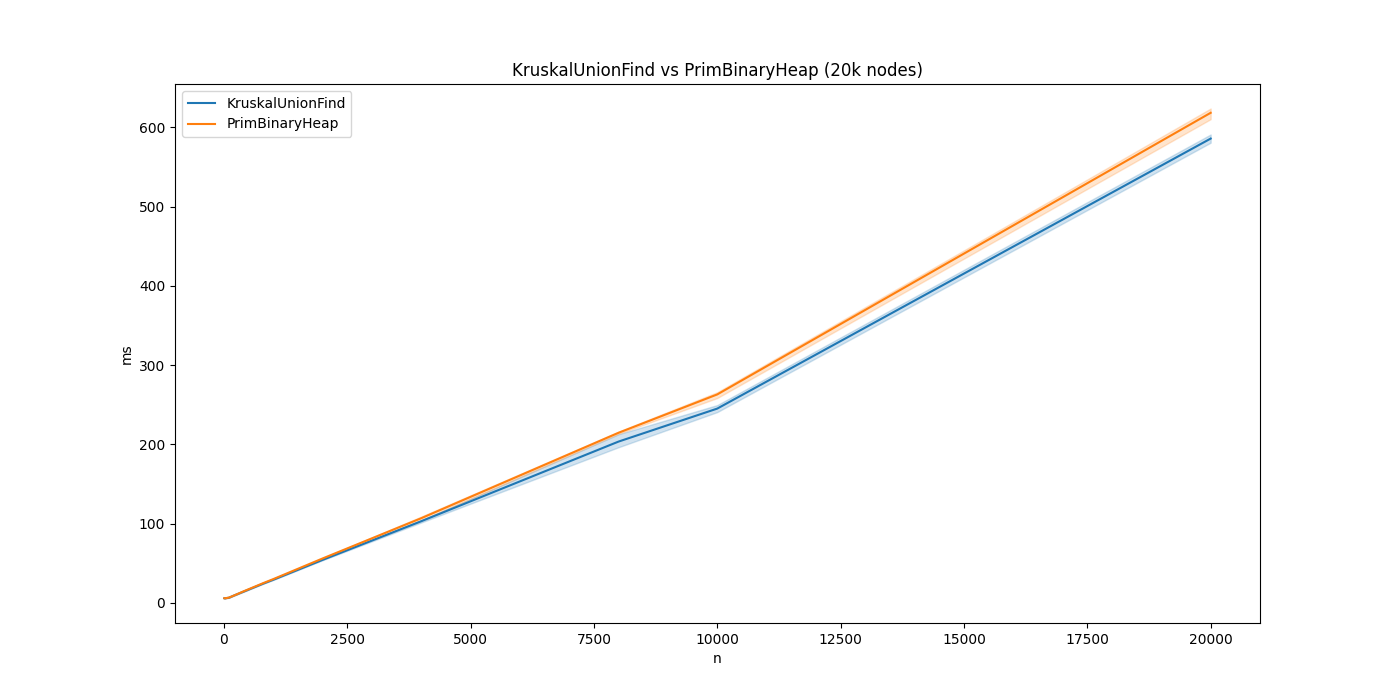
\includegraphics[width=1.0\textwidth]{./images/KruskalUnionFind_vs_PrimBinaryHeap_(20k_nodes).png}
    \caption{Andamento di KruskalUnionFind e PrimBinaryHeap con taglia dell'input da 0 a 20000 nodi.}
    \label{fig:TheTwoComparison5k}
\end{figure}

\subsection{Domanda \#2}

\begin{displayquote}
Commentate i risultati che avete ottenuto: come si comportano gli algoritmi rispetto alle varie istanze? C'è un algoritmo che riesce sempre a fare meglio degli altri? Quale dei tre algoritmi che avete implementato è più efficiente?
\end{displayquote}

\noindent Le tabelle \ref{table:kruskal-naive-vs-kruskal-union-find}, \ref{table:kruskal-naive-vs-kruskal-union-find-compressed}, \ref{table:kruskal-naive-vs-prim-binary-heap}, \ref{table:kruskal-union-find-vs-kruskal-union-find-compressed}, \ref{table:prim-binary-heap-vs-kruskal-union-find-compressed}, \ref{table:prim-binary-heap-vs-kruskal-union-find}, \ref{table:prim-binary-heap-vs-prim-k-heap}, \ref{table:prim-k-heap-vs-kruskal-union-find}, \ref{table:prim-k-heap-vs-kruskal-union-find-compressed} mostrano il confronto tra i millisecondi di esecuzione e il numero di nodi del grafo. Per motivazioni grafiche, abbiamo scelto gli scaglioni 8.000, 10.000, 20.000, 80.000, 100.000 come numero di nodi. \\

\noindent Dalle tabelle di confronto \ref{table:kruskal-naive-vs-kruskal-union-find}, \ref{table:prim-binary-heap-vs-kruskal-union-find} e \ref{table:prim-k-heap-vs-kruskal-union-find} è evidente che \textbf{KruskalUnionFind} è il più efficiente tra gli algoritmi di cui era richiesta l'implementazione. Inoltre, osservando la tabella di confronto \ref{table:kruskal-union-find-vs-kruskal-union-find-compressed}, è possibile notare che l'utilizzo della tecnica \textit{path-compression} nella struttura dati \textbf{Disjoint-Set} in realtà non abbia portato benefici, e anzi abbia peggiorato leggermente le performance (che sono comunque migliori di \textit{PrimBinaryHeap} e \textit{PrimKHeap}, vedasi le tabella di confronto \ref{table:prim-binary-heap-vs-kruskal-union-find-compressed} e \ref{table:prim-k-heap-vs-kruskal-union-find-compressed}). \\

\begin{table}[H]
\centering
    \begin{tabular}{|l|rrrrrr|}
    \hline
    &  \multicolumn{1}{c}{8k} & \multicolumn{1}{c}{10k} & \multicolumn{1}{c}{20k} & \multicolumn{1}{c}{20k} & \multicolumn{1}{c}{80k} &           \multicolumn{1}{c|}{100k} \\
    \hline
     KruskalNaive     & 3043.06  & 4865.46  & 24826.2   & 165997    & 757996    &    1209660.531 \\
     KruskalUnionFind &  194.548 &  249.867 &   592.052 &   1241.17 &   2935.21 & 3956.8         \\ \hline
     Differenza       & 2848.51  & 4615.6   & 24234.2   & 164756    & 755061    &    1205703.731  \\
     Miglioramento \%  &   93.61  &   94.86  &    97.62  &     99.25 &     99.61 &   99.67           \\
    \hline
    \end{tabular}
    \caption{Confronto tra KruskalNaive e KruskalUnionFind.}
    \label{table:kruskal-naive-vs-kruskal-union-find}
\end{table}

\begin{table}[H]
\centering
    \hspace*{-1cm}
    \begin{tabular}{|l|rrrrrr|}
    \hline
    &  \multicolumn{1}{c}{8k} & \multicolumn{1}{c}{10k} & \multicolumn{1}{c}{20k} & \multicolumn{1}{c}{20k} & \multicolumn{1}{c}{80k} &           \multicolumn{1}{c|}{100k} \\
    \hline
     KruskalNaive               & 3043.06  & 4865.46  & 24826.2   & 165997    & 757996    &    1209660.531 \\
     KruskalUnionFindCompressed &  203.831 &  249.867 &   594.038 &   1246.26 &   2935.21 & 3956.8         \\ \hline
     Differenza                 & 2839.23  & 4615.6   & 24232.2   & 164751    & 755061    &    1205703.731 \\
     Miglioramento \%            &   93.3   &   94.86  &    97.61  &     99.25 &     99.61 &   99.67          \\
    \hline
    \end{tabular}
    \caption{Confronto tra KruskalNaive e KruskalUnionFindCompressed.}
    \label{table:kruskal-naive-vs-kruskal-union-find-compressed}
\end{table}

\begin{table}[H]
\centering
    \begin{tabular}{|l|rrrrrr|}
    \hline
    &  \multicolumn{1}{c}{8k} & \multicolumn{1}{c}{10k} & \multicolumn{1}{c}{20k} & \multicolumn{1}{c}{20k} & \multicolumn{1}{c}{80k} &           \multicolumn{1}{c|}{100k} \\
    \hline
     KruskalNaive      & 3043.06  & 4865.46  & 24826.2   & 165997    & 757996   & 1209660.531 \\
     PrimBinaryHeap    &  217.068 &  256.007 &   623.884 &   1315.29 &   3007.6 & 4073.46        \\ \hline
     Differenza        & 2825.99  & 4609.45  & 24202.3   & 164682    & 754989   & 1205587.075 \\
     Miglioramento \%   &   92.87  &   94.74  &    97.49  &     99.21 &     99.6 &   99.66       \\
    \hline
    \end{tabular}
    \caption{Confronto tra KruskalNaive e PrimBinaryHeap.}
    \label{table:kruskal-naive-vs-prim-binary-heap}
\end{table}

\begin{table}[H]
\centering
    \hspace*{-0.25cm}
    \begin{tabular}{|l|rrrrrr|}
    \hline
    &  \multicolumn{1}{c}{8k} & \multicolumn{1}{c}{10k} & \multicolumn{1}{c}{20k} & \multicolumn{1}{c}{20k} & \multicolumn{1}{c}{80k} &           \multicolumn{1}{c|}{100k} \\
    \hline
     KruskalUnionFind           & 194.548 & 249.867 & 592.052 & 1241.17 & 2935.21 & 3956.8 \\
     KruskalUnionFindCompressed & 203.831 & 249.867 & 594.038 & 1246.26 & 2935.21 & 3956.8 \\ \hline
     Differenza                 &  -9.283 &   0     &  -1.986 &   -5.09 &    0    &    0   \\
     Miglioramento \%            &  -4.77  &   0     &  -0.34  &   -0.41 &    0    &    0     \\
    \hline
    \end{tabular}
    \caption{Confronto tra KruskalUnionFind e KruskalUnionFindCompressed.}
    \label{table:kruskal-union-find-vs-kruskal-union-find-compressed}
\end{table}

\begin{table}[H]
\centering
    \begin{tabular}{|l|rrrrrr|}
    \hline
    &  \multicolumn{1}{c}{8k} & \multicolumn{1}{c}{10k} & \multicolumn{1}{c}{20k} & \multicolumn{1}{c}{20k} & \multicolumn{1}{c}{80k} &           \multicolumn{1}{c|}{100k} \\
    \hline
     PrimBinaryHeap   & 217.068 & 256.007 & 623.884 & 1315.29  & 3007.6   & 4073.46  \\
     KruskalUnionFind & 194.548 & 249.867 & 592.052 & 1241.17  & 2935.21  & 3956.8   \\ \hline
     Differenza       &  22.52  &   6.14  &  31.832 &   74.119 &   72.386 &  116.656 \\
     Miglioramento \%  &  10.37  &   2.4   &   5.1   &    5.64  &    2.41  &    2.86 \\
    \hline
    \end{tabular}
    \caption{Confronto tra PrimBinaryHeap e KruskalUnionFind.}
    \label{table:prim-binary-heap-vs-kruskal-union-find}
\end{table}

\begin{table}[H]
\centering
    \begin{tabular}{|l|rrrrrr|}
    \hline
    &  \multicolumn{1}{c}{8k} & \multicolumn{1}{c}{10k} & \multicolumn{1}{c}{20k} & \multicolumn{1}{c}{20k} & \multicolumn{1}{c}{80k} &           \multicolumn{1}{c|}{100k} \\
    \hline
 PrimBinaryHeap             & 217.068 & 256.007 & 623.884 & 1315.29  & 3007.6   & 4073.46  \\
 KruskalUnionFindCompressed & 203.831 & 249.867 & 594.038 & 1246.26  & 2935.21  & 3956.8   \\ \hline
     Differenza             &  13.237 &   6.14  &  29.846 &   69.029 &   72.386 &  116.656 \\
     Miglioramento \%        &   6.1   &   2.4   &   4.78  &    5.25  &    2.41  &    2.86  \\
    \hline
    \end{tabular}
    \caption{Confronto tra PrimBinaryHeap e KruskalUnionFindCompressed.}
    \label{table:prim-binary-heap-vs-kruskal-union-find-compressed}
\end{table}

\begin{table}[H]
\centering
    \begin{tabular}{|l|rrrrrr|}
    \hline
    &  \multicolumn{1}{c}{8k} & \multicolumn{1}{c}{10k} & \multicolumn{1}{c}{20k} & \multicolumn{1}{c}{20k} & \multicolumn{1}{c}{80k} &           \multicolumn{1}{c|}{100k} \\
    \hline
PrimBinaryHeap    & 217.068 & 256.007 & 623.884 & 1315.29  & 3007.6   & 4073.46  \\
PrimKHeap         & 214.689 & 266.522 & 622.871 & 1305.54  & 3092.63  & 4104.52  \\ \hline
Differenza        &   2.379 & -10.515 &   1.013 &    9.747 &  -85.032 &  -31.063 \\
Miglioramento \%  &   1.1   &  -4.11  &   0.16  &    0.74  &   -2.83  &   -0.76  \\
    \hline
    \end{tabular}
    \caption{Confronto tra PrimBinaryHeap e PrimKHeap.}
    \label{table:prim-binary-heap-vs-prim-k-heap}
\end{table}

\begin{table}[H]
\centering
    \begin{tabular}{|l|rrrrrr|}
    \hline
    &  \multicolumn{1}{c}{8k} & \multicolumn{1}{c}{10k} & \multicolumn{1}{c}{20k} & \multicolumn{1}{c}{20k} & \multicolumn{1}{c}{80k} &           \multicolumn{1}{c|}{100k} \\
    \hline
PrimKHeap        & 214.689 & 266.522 & 622.871 & 1305.54  & 3092.63  & 4104.52  \\
KruskalUnionFind & 194.548 & 249.867 & 592.052 & 1241.17  & 2935.21  & 3956.8   \\ \hline
Differenza       &  20.141 &  16.655 &  30.819 &   64.372 &  157.418 &  147.719 \\
Miglioramento \%    &   9.38  &   6.25  &   4.95  &    4.93  &    5.09  &    3.6   \\
    \hline
    \end{tabular}
    \caption{Confronto tra PrimKHeap e KruskalUnionFind.}
    \label{table:prim-k-heap-vs-kruskal-union-find}
\end{table}

\begin{table}[H]
\centering
    \begin{tabular}{|l|rrrrrr|}
    \hline
    &  \multicolumn{1}{c}{8k} & \multicolumn{1}{c}{10k} & \multicolumn{1}{c}{20k} & \multicolumn{1}{c}{20k} & \multicolumn{1}{c}{80k} &           \multicolumn{1}{c|}{100k} \\
    \hline
PrimKHeap                  & 214.689 & 266.522 & 622.871 & 1305.54  & 3092.63  & 4104.52  \\
KruskalUnionFindCompressed & 203.831 & 249.867 & 594.038 & 1246.26  & 2935.21  & 3956.8   \\ \hline
Differenza                 &  10.858 &  16.655 &  28.833 &   59.282 &  157.418 &  147.719 \\
Miglioramento \%           &   5.06  &   6.25  &   4.63  &    4.54  &    5.09  &    3.6   \\
    \hline
    \end{tabular}
    \caption{Confronto tra PrimKHeap e KruskalUnionFindCompressed.}
    \label{table:prim-k-heap-vs-kruskal-union-find-compressed}
\end{table}
% \paragraph{Premessa}\mbox{} \\

% È doveroso notare che nei dataset a disposizione non esiste alcun grafo il cui numero di archi $m$ sia maggiore del numero di vertici $n$ per più di un fattore 1.5 (ovvero, $m = $ \complexityN{}). In questo homework abbiamo quindi avuto a che fare con grafi sparsi. Poiché l'algoritmo Kruskal con Disjoint-Set ha complessità \complexityMLogN{} e

\noindent In teoria, KruskalUnionFindCompressed avrebbe dovuto essere l'algoritmo più efficiente di tutti, con complessità temporale \complexityKruskalCompressed{}, ovvero \complexityMLogM{} (o, equivalentemente, \complexityMLogN{}).

\noindent PrimBinaryHeap e KruskalUnionFind hanno la stessa complessità temporale teorica \newline (\complexityMLogN{}), ma in realtà le operazioni del BinaryHeap hanno un coefficiente di complessità più elevato rispetto a quelle della struttura dati Disjoint-Set, per cui KruskalUnionFind risulta essere più veloce. \\

\noindent Infine, data la complessità teorica elevata di KruskalNaive (\complexityMN{}), avevamo già ipotizzato che sarebbe stato l'algoritmo più lento tra quelli implementati. Tale assunzione è poi stata confermata dall'analisi pratica effettuata. \\

\noindent Non abbiamo un'idea certa del perché Kruskal implementato con \textit{DisjointSetCompressed} sia meno performante di \textit{DisjointSet}. La nostra ipotesi è che, per gli input forniti al nostro programma, il \textit{cache behaviour} di KruskalUnionFind sia molto migliore di quello di KruskalUnionFindCompressed.
